\section{Implementa��o}
\label{implementacao}

A Figura \ref{fig:bibliotecas} apresenta as camadas do sistema, bem como as bibliotecas utilizadas.

\begin{figure}[h]
	\center{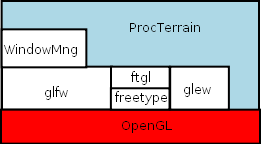
\includegraphics[width=0.6\linewidth]{img/bibliotecas.png}}
	\caption{\label{fig:bibliotecas} Camadas do sistema.}
\end{figure}

A camada \emph{WindowMng} tem como prop�sito simular a um aplicativo gr�fico gen�rico (\emph{game}, simulador, etc.); desta forma, o sistema poder� ser posteriormente adaptado para funcionar em conjunto com outros aplicativos que possam ser desenvolvidos (ou acoplado a uma \emph{engine}).

A Figura \ref{fig:arquitetura} apresenta em detalhes os m�dulos presentes nas camadas \emph{WindowMng} e \emph{ProcTerrain}. A seguir, uma explica��o sobre cada um dos m�dulos.

\begin{figure}[h]
	\center{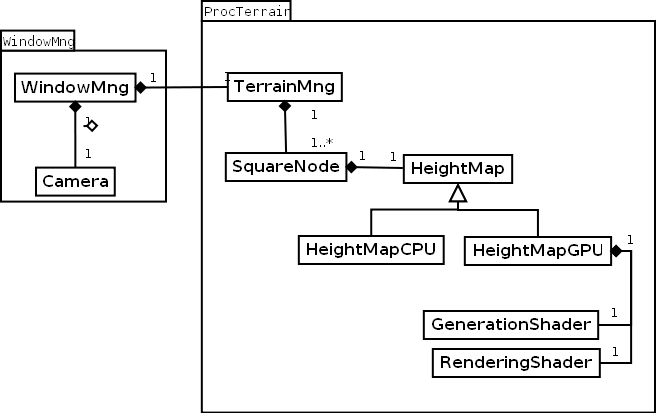
\includegraphics[width=0.6\linewidth]{img/arquitetura.png}}
	\caption{\label{fig:arquitetura} Diagrama com as principais classes do sistema implementado.}
\end{figure}

\begin{itemize}
	\item {\bf WindowMng}: Respons�vel por simular um aplicativo gr�fico gen�rico, e chamar os devidos \emph{callbacks} do pacote \emph{ProcTerrain}.
	\item {\bf Camera}: M�dulo que implementa uma c�mera controlada pelo jogador e navegando pelo mundo.
	\item {\bf TerrainMng}: M�dulo respons�vel por gerar e controlar os terrenos.
	\item {\bf SquareNode}: Nodo que representa uma fatia (\emph{patch}) do terreno.
	\item {\bf HeightMap}: M�dulo que implementa os mapas de altura dos terrenos gerados na CPU ou na GPU.
	\item {\bf GenerationShader}: \emph{Shader} respons�vel pela gera��o dos terrenos.
	\item {\bf RenderingShader}: \emph{Shader} respons�vel pela renderiza��o dos terrenos.
\end{itemize}
